\documentclass[a4paper, english, 12pt]{article}

% General packages
\usepackage{parskip}      % Vertical space on new paragraph instead of indent
\usepackage{hyperref}   % For including links
\usepackage{url}          % Allows adding url's
\usepackage[top=4cm, bottom=4cm]{geometry}     % Easier management of page dimensions
\usepackage{chngcntr}     % Customizable counters
\usepackage{enumitem}     % Can use [noitemsep] on lists to reduce spacing
\usepackage{fancyhdr}
\pagestyle{fancy}
\usepackage{afterpage} 	% Various tweaks for page breaks and stuff

% BEGIN Floats
\usepackage[bf, hang, small]{caption}	% Nicer captions for floats.
\usepackage{float}        % Allows advanced placement options for floats
% \usepackage{subfig}		% Sub-figures. Crashes with captions package
% END Floats


% BEGIN Tables
\usepackage{booktabs}		% More professional looking tables
\usepackage{tabularx}		% Allows width adjustment etc. for tables
\usepackage{multirow}		% Allows table cells to span rows or columns




% Font specific packages
\usepackage{fontspec}
\usepackage{textcomp}
\usepackage{titlesec}
\usepackage{titling}
\usepackage{inconsolata}
\usepackage[default]{droidserif}

% Specifying fonts
\setsansfont{Open Sans}
\setmainfont[Scale=0.80]{Droid Serif}
\fontspec{Inconsolata}
\setmonofont[Scale=0.80]{Inconsolata}
\newfontfamily\headingfont[]{Open Sans}
\newfontfamily\headingfont[]{Open Sans}
\titleformat*{\section}{\Large\headingfont}
\titleformat*{\subsection}{\large\headingfont}
\titleformat*{\subsubsection}{\normalsize\headingfont}
\renewcommand{\maketitlehooka}{\headingfont}



\usepackage{moreverb}     % Allows use of tables in verbatim
\usepackage{fancyvrb}     % Fancy verbatim stuff
\usepackage{listings}     % Source code listings
\usepackage[usenames,dvipsnames]{color}		% Used for colors by various other packages

% Configuring listings
\definecolor{light-gray}{RGB}{250,250,250} 	% Background color for listings
\definecolor{gray}{RGB}{100,100,100} 	% Color for line-numbers
\lstset{
	language={C},			% the language of the code
	aboveskip=1em,
	belowskip=-3em,
	basicstyle=\ttfamily\footnotesize,
	backgroundcolor=\color{light-gray},
	frame=single,				% adds a frame around the code
	rulecolor=\color{black},	% frame color
	captionpos=t,				% sets the caption-position to bottom
	breaklines=true,			% sets automatic line breaking
	breakatwhitespace=false,	% automatic breaks only at whitespace?
	keepspaces=true,			% keeps spaces in text, useful for keeping indentation of code (possibly needs columns=flexible)
	tabsize=4,					% sets default tabsize to 2 spaces
	commentstyle=\color{green},	% comment style
	keywordstyle=\color{blue},	% keyword style
	stringstyle=\color{red},	% string literal style
	numbers=left,				% line-number position: none, left or right
	numbersep=5pt,				% how far the line-numbers are from the code
	numberstyle=\tiny\color{gray}, % the style that used for line-numbers
	stepnumber=2,				% step between two line-numbers.
	showspaces=false,			% show spaces everywhere with underscores
	showtabs=false,				% show tabs within strings with underscores
	showstringspaces=false,		% underline spaces within strings only
	escapeinside={\%*}{*)},		% if you want to add LaTeX within your code
	title=\lstname				% show the filename of files included with \lstinputlisting; also try caption instead of title
}

\usepackage{cite}



\title{3D Visualization of petroleum data\\ 
\vspace{6pt}\large Exercise 3: Color mapping \\ 
 }
\author{Einar Baumann}   
\date{\today}


\begin{document}

\maketitle
\thispagestyle{empty}
\pagebreak

\section{Setup}
\label{sec:setup}
As I am using Linux and not Windows, the recommended tutorial was not of much help for getting started. Instead I used a tutorial I found on the OpenGL Wiki \cite{gltutorial}. This tutorial recommend that I used \emph{GLX} and \emph{Xlib} to enable displaying OpenGL using the X Window system, which is the default window system for most Linux distributions.

I used the framework laid out in the tutorial (with some tweaking) to build my application, substituting my own OpenGL commands.

I used plain C for the implementation, as it's what I'll have to do for a project in a very similar course I'm taking parallel to this course.
% section setup (end)

\section{Drawing the squares}
\label{sec:drawing}
For drawing the squares, I used a \emph{Vertex Array Object}, which is now the standard way of doing such things, after the \texttt{glBegin} / \texttt{glEnd} structure was deprecated. A vertex array object encapsulates all of the state needed to specify vertex data, including the format of the vertex data (e.g. quads, triangles, polygons) and the sources for the vertex arrays.

\emph{Vertex Buffer Objects} were not used, as the program only contains one instance of one object. 
% section drawing (end)

\section{Color mapping}
\label{sec:color_mapping}
I used a \emph{Color Array} to map colors onto the squares. The array defining the colors were generated using the scalar algorithm outlined in the course to map the temperatures given for the vertices onto the given colors.

The algorithm relies on a specified set of \emph{n} colors in a zero-indexed list, as well as knowing the \emph{min} and \emph{max} values in our range. We input this, along with the value $s_i$ that we wish to map, into equation (\ref{eq:algorithm}) to calculate an index \emph{i}. The index points us to one of the \emph{n} defined colors.

\begin{equation}
	\label{eq:algorithm}
	i = n \left( \frac{s_i - min}{max - min} \right)
\end{equation}

The result of the color mapping is shown in Figures \ref{fig:symmetry-1} and \ref{fig:symmetry-2}.
% section color_mapping (end)

\section{Symmetry}
\label{sec:symmetry}
First off, GL\_QUADS has been deprecated since OpenGL v3.1 -- this is due to the fact that GPU's are optimized for rendering triangles. Even when using GL\_QUADS, the squares are decomposed into two triangles. As far as I can see, what is done is roughly equivalent to placing an extra edge between the first and the third vertex that is drawn according to the index list.

If two vertices have the same color and an edge connecting them, the entire edge will have the same constant color as the vertices; i.e. there is no real interpolation along the center of it. This is seen in Figure \ref{fig:symmetry-2}. This results in an unnatural-looking temperature distribution on our case.

In the symmetry seen in Figure \ref{fig:symmetry-1} we can still see the edges created when the two squares are decomposed (and of course the center edge), but the resulting interpolation looks -- to me at least -- more natural.
\begin{figure}[p]
\centering
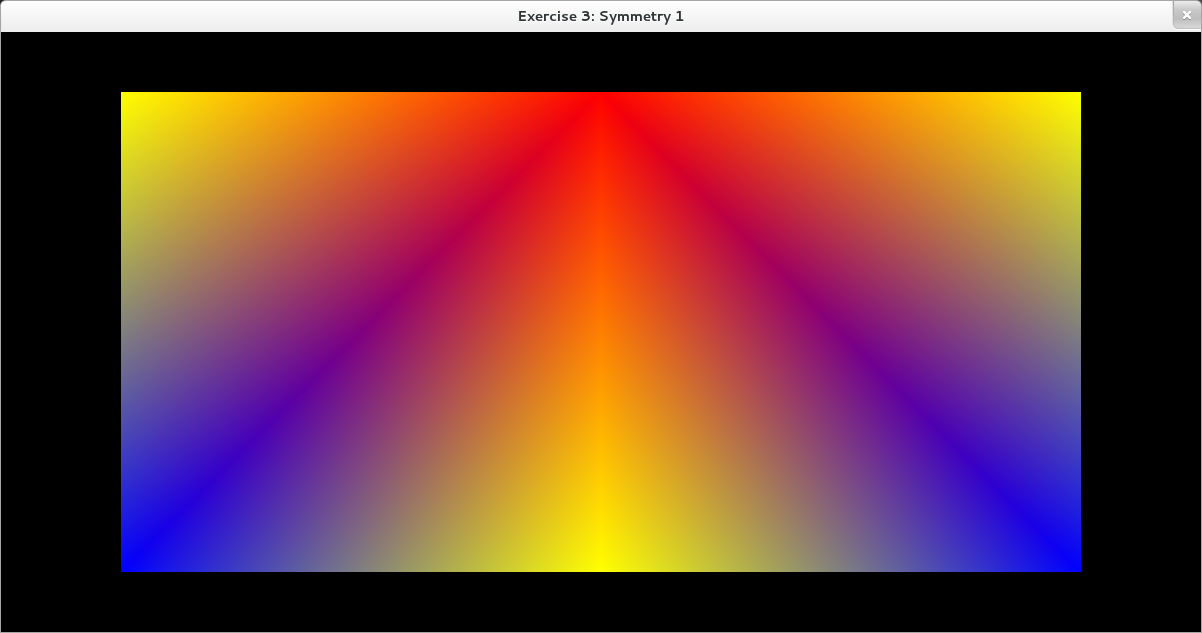
\includegraphics[width=\textwidth]{figures/symmetry-1.png}
\caption{A screen-cap of the first of two possible configurations with symmetry along the vertical center line.}
\label{fig:symmetry-1}
\end{figure}

\begin{figure}[p]
\centering
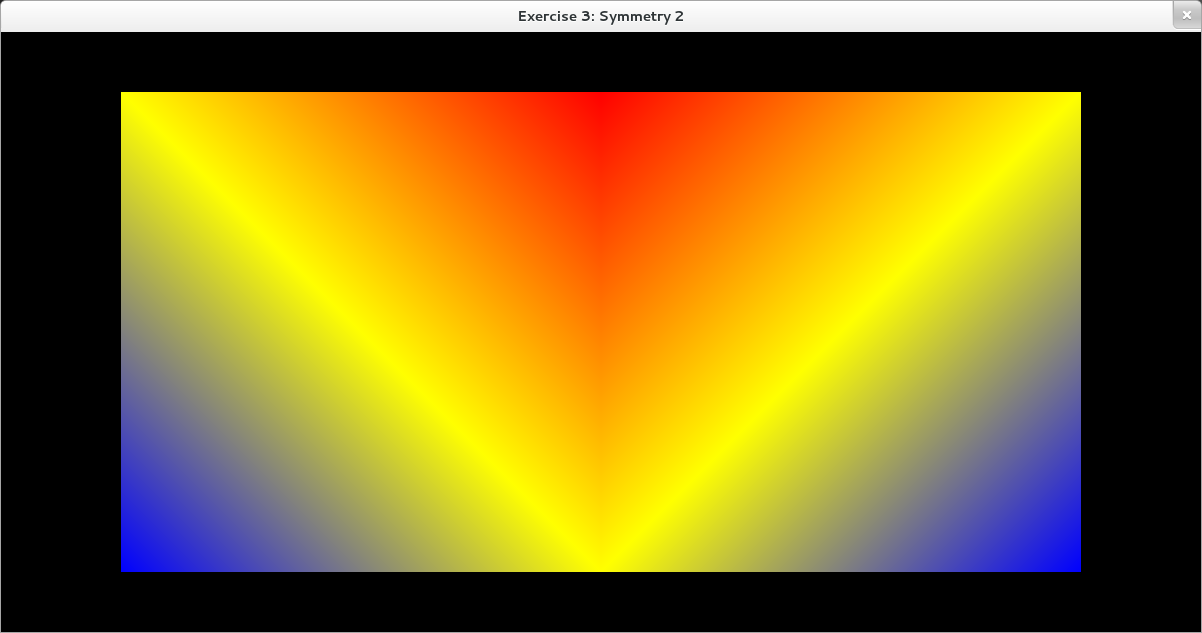
\includegraphics[width=\textwidth]{figures/symmetry-2.png}
\caption{A screen-cap of the second of two possible configurations with symmetry along the vertical center line.}
\label{fig:symmetry-2}
\end{figure}

% section symmetry (end)

\pagebreak
\bibliography{references.bib}{}
\bibliographystyle{plain}


\pagebreak
\appendix
\section{Source code}
\label{sec:app_source}

\subsection{Main program}
\label{sub:source_main}
\lstinputlisting[title=ex3-colorquads.c]{../ex3-colorquads.c}
% subsection  (end)

\subsection{OpenGL and X commands}
\label{sub:source_gl}
\lstinputlisting[title=ex3-glfuns.c]{../ex3-glfuns.c}
% subsection  (end)

% section  (end)

\end{document}















































